\documentclass[11pt, a4paper]{article}
\usepackage[utf8]{inputenc}
\usepackage{amsmath, amssymb}
\usepackage{graphicx}
\usepackage{hyperref}
\usepackage{xcolor}
\usepackage{listings}
\lstset{
    language=Python,
    basicstyle=\ttfamily\small,
    keywordstyle=\color{blue}\bfseries,
    commentstyle=\color{gray}\itshape,
    stringstyle=\color{orange},
    numberstyle=\tiny\color{gray},
    numbers=left,
    stepnumber=1,
    numbersep=8pt,
    frame=single,
    breaklines=true,
    breakatwhitespace=false,
    showstringspaces=false,
    tabsize=4,
    captionpos=b
}
\usepackage{geometry}
\geometry{margin=1in}

\title{EE 325 Digital Signal Processing \\ Assignment 7: Stability of Discrete-Time Systems}
\author{PERERA J.D.T. \\ E/21/291}
\date{\today}

\begin{document}
\maketitle

\section{1. BIBO Stability from Impulse Response}
A linear time-invariant (LTI) system is BIBO stable if and only if the impulse response is absolutely summable:
$$ \sum_{n=-\infty}^{\infty} |h[n]| < \infty $$

\subsection{(a) $h_1[n] = 2^n u[n]$}
$$ \sum_{n=-\infty}^{\infty} |2^n u[n]| = \sum_{n=0}^{\infty} 2^n = 1 + 2 + 4 + \dots = \infty $$
\textbf{Conclusion:} Unstable. The sum diverges.

\subsection{(b) $h_2[n] = (-0.5)^n u[n]$}
$$ \sum_{n=-\infty}^{\infty} |(-0.5)^n u[n]| = \sum_{n=0}^{\infty} |(-0.5)|^n = \sum_{n=0}^{\infty} (0.5)^n $$
Using geometric series sum $\sum_{n=0}^{\infty} r^n = \frac{1}{1-r}$ for $|r| < 1$:
$$ \sum_{n=0}^{\infty} (0.5)^n = \frac{1}{1-0.5} = \frac{1}{0.5} = 2 < \infty $$
\textbf{Conclusion:} Stable. The sum is finite.

\subsection{(c) $h_3[n] = u[n]$}
$$ \sum_{n=-\infty}^{\infty} |u[n]| = \sum_{n=0}^{\infty} 1 = 1 + 1 + 1 + \dots = \infty $$
\textbf{Conclusion:} Unstable. The sum diverges.

\section{2. Jury Stability Test}

Characteristic polynomial: $p(z) = z^2 - 1.7z + 0.6$. \\
Coefficients: $a_2 = 1, a_1 = -1.7, a_0 = 0.6$.

\subsection{(a) Jury Table and Conditions}
For a 2nd order system ($N=2$), the necessary and sufficient conditions for stability are:
\begin{enumerate}
    \item $P(1) > 0$
    \item $(-1)^2 P(-1) > 0 \Rightarrow P(-1) > 0$
    \item $|a_0| < a_2$ (assuming $a_2 > 0$)
\end{enumerate}

\textbf{Checking Conditions:}
\begin{enumerate}
    \item $P(1) = (1)^2 - 1.7(1) + 0.6 = 1 - 1.7 + 0.6 = -0.1$ \\
    Condition $P(1) > 0$ is \textbf{FALSE}.
    \item $P(-1) = (-1)^2 - 1.7(-1) + 0.6 = 1 + 1.7 + 0.6 = 3.3$ \\
    Condition $P(-1) > 0$ is \textbf{TRUE}.
    \item $|a_0| < a_2 \Rightarrow |0.6| < 1$ \\
    Condition is \textbf{TRUE}.
\end{enumerate}

\textbf{Conclusion:} Since the first condition fails ($P(1) = -0.1 \ngtr 0$), the system is \textbf{UNSTABLE}.

\subsection{(b) Verification with Roots}
Roots of $z^2 - 1.7z + 0.6 = 0$:
$$ z = \frac{1.7 \pm \sqrt{(-1.7)^2 - 4(1)(0.6)}}{2} = \frac{1.7 \pm \sqrt{2.89 - 2.4}}{2} $$
$$ z = \frac{1.7 \pm \sqrt{0.49}}{2} = \frac{1.7 \pm 0.7}{2} $$
$$ z_1 = \frac{2.4}{2} = 1.2, \quad z_2 = \frac{1.0}{2} = 0.5 $$
Only stable if all poles satisfy $|z| < 1$. \\
Here, $|z_1| = 1.2 > 1$. \\
\textbf{Conclusion:} The system is \textbf{UNSTABLE}, consistent with the Jury test.

\section{3. System Behavior Analysis}
\begin{itemize}
    \item \textbf{System A:} $y[n] - 0.5y[n-1] = x[n]$
    \begin{itemize}
        \item Characteristic equation: $z - 0.5 = 0 \Rightarrow z = 0.5$.
        \item Since $|z| = 0.5 < 1$, the pole is inside the unit circle.
        \item \textbf{Expectation:} Stable system, bounded output for bounded input.
    \end{itemize}
    \item \textbf{System B:} $y[n] - 1.2y[n-1] = x[n]$
    \begin{itemize}
        \item Characteristic equation: $z - 1.2 = 0 \Rightarrow z = 1.2$.
        \item Since $|z| = 1.2 > 1$, the pole is outside the unit circle.
        \item \textbf{Expectation:} Unstable system, unbounded output (exponential growth) for bounded input.
    \end{itemize}
\end{itemize}

\begin{figure}[h]
    \centering
    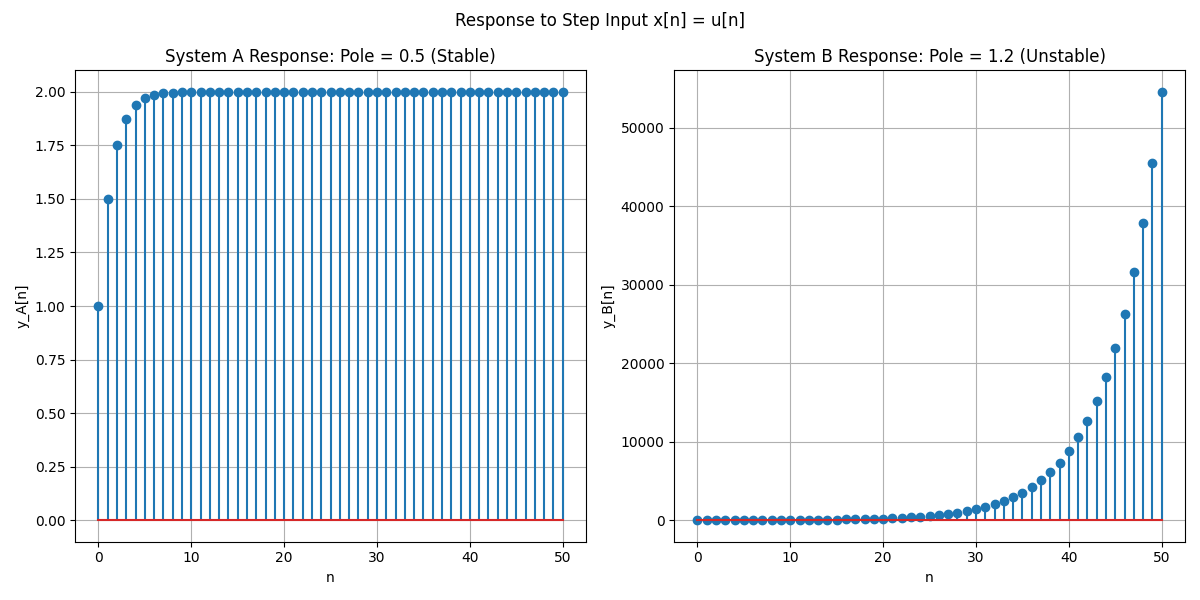
\includegraphics[width=1\textwidth]{plots/system_responses.png}
    \caption{System Responses Verification}
    \label{fig:sys_res}
\end{figure}

\appendix
\section{Python Source Code}
\textbf{File:} \texttt{assignment7\_sim.py}
\begin{lstlisting}[caption={Stability Simulation: Stable vs. Unstable Systems -- Assignment 7}]
import numpy as np
import matplotlib.pyplot as plt
from scipy.signal import lfilter
import os

def run_simulation():
    if not os.path.exists('plots'):
        os.makedirs('plots')

    n = np.arange(0, 51)
    x = np.ones_like(n)  # Unit Step input

    # System A: pole at 0.5 (stable)
    b_A = [1.0]
    a_A = [1.0, -0.5]
    y_A = lfilter(b_A, a_A, x)

    # System B: pole at 1.2 (unstable)
    b_B = [1.0]
    a_B = [1.0, -1.2]
    y_B = lfilter(b_B, a_B, x)

    plt.figure(figsize=(12, 6))
    plt.subplot(1, 2, 1)
    plt.stem(n, y_A)
    plt.title('System A Response: Pole = 0.5 (Stable)')
    plt.xlabel('n')
    plt.ylabel('y_A[n]')
    plt.grid(True)

    plt.subplot(1, 2, 2)
    plt.stem(n, y_B)
    plt.title('System B Response: Pole = 1.2 (Unstable)')
    plt.xlabel('n')
    plt.ylabel('y_B[n]')
    plt.grid(True)

    plt.suptitle('Response to Step Input x[n] = u[n]')
    plt.tight_layout()
    output_path = os.path.join('plots', 'system_responses.png')
    plt.savefig(output_path)
    print(f"Plot saved to {output_path}")

if __name__ == "__main__":
    run_simulation()
\end{lstlisting}

\end{document}
